\documentclass{bioinfo}
\copyrightyear{2014}
\pubyear{2014}




%%% Additional Macro and command.
\usepackage{url}
\newcommand{\pkg}[1]{{\fontseries{b}\selectfont #1}}
\makeatletter
\newcommand\code{\bgroup\@makeother\_\@makeother\~\@makeother\$\@codex}
\def\@codex#1{{\normalfont\ttfamily\hyphenchar\font=-1 #1}\egroup}
\makeatother
\let\proglang=\textsf
%%% End of additional Macro and command.


\newcommand{\package}{ribModel } % need that whitespace there for text flow


%%% Start here.
\begin{document}
\firstpage{1}

\title[ribModel]{ribModel: extracting biological information from codon usage data}
\author[
Landerer \textit{et~al}]{Cedric Landerer\,$^{1,3}$\footnote{
to whom correspondence should be addressed
},
Alex Cope\,$^{4,5}$
Russell Zaretzki\,$^{2,3}$, and
Michael Gilchrist\,$^{1,3}$
}
\address{$^{1}$
Department of Ecology and Evolutionary Biology,
$^{2}$Department of Statistics, Operations, and Management Science, and
$^{3}$National Institute for Mathematical and Biological Synthesis,
University of Tennessee, Knoxville, TN, USA,
$^{4}$Genome Science and Technology, University of Tennessee, Knoxville, TN, USA
$^{5}$Oak Ridge National Labratory, Oak Ridge, TN, USA} 
\history{Received on XXXXX; revised on XXXXX; accepted on XXXXX}

\editor{Associate Editor: XXXXXXX}

\maketitle

\begin{abstract}

\section{Summary:}
\pkg{\package} is a collection of codon models, estimating terms related to mutation and selection coefficients of synonymous codon usage bias (CUB) and population genetics parameters of interest. 
The implemented models allow users to analyze sequence data and ribosome foot printing data to estimate selection on ribosome overhead costs, nonsense error rates, and ribosome pausing times. 
\package also allows for the estimation of the evolutionary average protein synthesis rate, reflecting the environmental conditions an organism evolves under. 
The framework provides an R interface for ease of use and is implemented with a generic design to allow for addition to current and future codon models.

\section{Availability:}
\pkg{\package} and documents are freely available under the Mozilla Public License 2.0
on CRAN (\url{http://cran.r-project.org/package=cubfits}).

\section{Contact:} \href{cedric.landerer@gmail.com}{cedric.landerer@gmail.com}
\end{abstract}


%\section*{Introduction}

%\begin{itemize}
%\item Huge influx of genome scale data sets across the tree of life
%\item Why study CUB?
%	\begin{itemize}
%	\item CUB is shaped by mutation and selection
%	\item informs about selection on translation efficiency.
%	\item translation efficiency can mean ribosome pausing, error free translation (nonsense or missense errors).
%	\item CUB potentially relates to co-translational folding. Tools allows to get at questions
%	\end{itemize}
%\item compare to CAI and tAI
%	\begin{itemize}
%	\item CAI and such require reference set of house-keeping gens for comparison of adaptation
%	\item tAI uses tRNA copy number implying no other factors are involved
%	\item We have population genetics component getting at $N_e * s$ with our model
%	\end{itemize}
%\item inference of expression as evolutionary mean unaffected by growth conditions and experimental noise
%\item Bayesian MCMC method allows for priors and multilevel and hierarchy 
%\end{itemize}



%\section*{Results}
%\begin{itemize}
%\item Performance (simulated data)
%	\begin{itemize}
%	\item runtime by number of genes and number of mixtures
%	\item confidence in parameters by number of genes
%	\item estimation of phi values (gene ordering)
%	\end{itemize}
%\item $s_{epsilon}$ as a measure of noise due to the lab conditions by eliminating technical 			noise. Use replicates to estimates technical noise
%\end{itemize}


\section*{Introduction}
Improvements in DNA sequencing technology and methodolgy allowed for an exponential growth in the number of publicly availble genomes over the past 15 years.
This influx of data necessitates the development of computational tools which allow researchers to extract biological information.

Information regarding selection on the translation process, such as factors shaping translational efficiency and co-translational folding, can be extracted from codon usage bias (CUB) data.
CUB refers to non-uniform usage of synonymous codons shaped by biases in mutation and selection.
Although CUB was first studied almost 40 years ago, many questions related to the factors shaping CUB remain open.
As a result, many metrics were developed in an attempt to quantify CUB, such as the Codon Adaptation Index (CAI).
CAI and similar metrics often take a selection-driven perspective when quantifying CUB. For example, CAI uses a set of supposedly highly expressed genes, such as ribosomal protein coding genes, to determine the "optimal" codons. This approach implicitly biases the results as they are not based the entire set protein-coding genes. 
Recent work demonstrated quantification of CUB is significantly improved in a population genetics context, which allows for both adaptive and non-adaptive evolutionary processes to be accounted for in shaping CUB.
[Gilchrist et al 2015] described a mechanistic model rooted in population genetics which accounted for selection, mutation bias, and genetic drift in quantifying CUB. From this model, which we call the Ribosomal Overhead Cost Stochastic Evolutionary Model of Protein Production Rates (ROC SEMPPR), relative values of selection for translational efficiency and mutation bias within each synonymous codon family could be estimated. The influence of adaptive and non-adaptive processes on CUB is shaped by the evolutionary average protein production rate of a gene. Genes with increased protein productions rates are belived to be under higher selection for translation efficiency and are therefore composed of a higher percentage of translationally-efficient codons. The relationship between these three biological parameters (selection, mutation bias, and protein production rates) allows ROC SEMPPR to also provide accurate estimates of protein production production rates. 
Here, we describe an open-source computational tool that allows researchers to analyze CUB data using ROC SEMPPR presented in [Gilchrist et al 2015]. This implementation builds off the previous work by introducing a mixture model for the selection and mutation bias parameters. In addition to the ROC SEMPPR model, additional models for extracting biological information from codon usage data are included in the package.


\begin{figure*}[!tpb]
\centering
 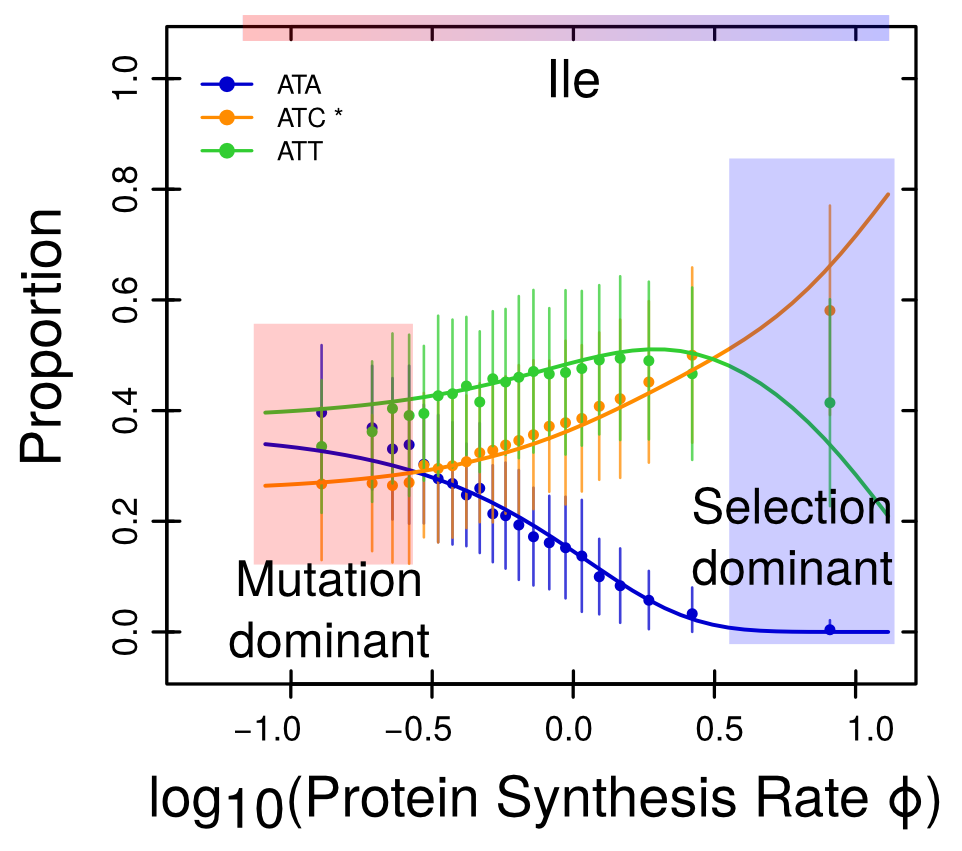
\includegraphics[width=3.5in]{expl_model.png}
\vspace{-0.2cm}
\caption{Binning for amino acid Isoleucine by expression levels (y-axis) where dots are mean proportions of synonymous codons (x-axis) of 100 simulated sequences in every 5\% expression windows, and vertical lines are 90\% empirical intervals. The curves are theoretical prediction of codon usages.
}
\label{fig:plotbin}
\end{figure*}

\section*{Features}
The \package interface is written in R, a freely available programming language noted for its ease of use for even inexperienced programmers. As a result, \package is accessible to researchers with minimal computational experience. The provided framework was designed to allow researchers to analyze their data swiftly without the need for long pre-processing of data sets. Generally, the only input needed for fitting a model to the data are protein-coding nucleotide sequences in the form of a FASTA file. If available, users may also provide empirically estimated values of gene expression as additional information for the model. However, this is not required.
\package also provides visualization functionality, including plots that compare parameter estimates across mixture categories (see below) and plots similar to Figure 1, which shows how codon usage varies with gene expression.    

\subsubsection*{Mixture distributions}
Mixture distributions are commonly used when the same data contains subpopulations which can be described by separate distributions with different parameter sets, (Gelman \textit{et al}, 2013). \package extends the ROC-SEMPPR model by allowing for a mixture distribution in the mutation and selection terms. This approach allows genes to be categorized based on differences in codon usage patterns, making \package ideal to answer questions about intra-genomic or even within-gene CUB heterogeneity.  

\subsubsection*{C++ to improve computational efficiency}
Although the \package interface is written in R, the functionality is written in C++ to improve computational performance.  
R does not provide a native C++ support; therfore we utilized the R package Rcpp (Eddelbuettel \& Francois 2011). 
Rcpp provides a module structure allowing the exposure of whole C++ classes to R. This minimizes data transfer between the R environment and the C++ core, resulting in improved computational performance. 
The runtime of \package scales linearly with genome size and iterations and XX with the increase of mixture distributions in the data set.

\subsubsection*{Writing extensions}
The object-oriented paradigm of C++ allowed for the implementation of a general framework for creating new models to analyze genomic data, (Booch 1993). All implemented models in \package are encapsulated such that they share certain commonalities. This allows for the creation of new models within the same framework. Generally, these models can be added by creating appropriate subclasses of the Parameter and Model classes provided by the current framework. These subclasses should include the additional functionality required for these models. \textbf{Alex: Overall, I think what I have here is pretty weak, but I don't have any better ideas at the moment.} 

\subsubsection*{Additional Models Available in \package}
\textbf{Alex: I currently do not know enough about these to write about them in detail}


\section*{Discussion}
\begin{itemize}
\item Runtime, scalability
\item Extendability, FONSE, PANSE, RFP
\item applications, hybridization, phylogenetics, variation in mutation and selection

\package provides researchers with an easy-to-use tool for extracting biological information from CUB data. Although the calculations in these models are not quite as straightforward as CAI and similar metrics of CUB, the population genetics roots of the models described allows for a clear, biological interpretation of their output. In addition, despite greater complexity in terms of calculations, runtime is generally not on an order of magnitude that will significnatly halt research progress.
The generic framework of \package makes it straight-forward to incorporate new functionality on either the R or the C++ side. Researchers developing new codon models are invited and welcome to incorporate them into \package.   
This package has many potential applications that might not be immediately apparent. The mixture model implementation has allowed for the examination of intra-genomic codon usage heterogeneity. \textbf{To Cedric: Maybe you could talk about some of the C left work here?} The mixture model implementation also allowed for a recent examination of codon usage variation in different sections within genes. 
\textbf{Alex: How do we want to end this? Probably need to make a broad statement about the usefulness of \package that will really sell it to the reader.} 


\end{itemize}



%\bibliographystyle{natbib}
%\bibliography{bioinfo}
\end{document}
